\documentclass[10pt,xcolor={usenames},fleqn,mathserif,serif]{beamer}

%% colors
\definecolor{bittersweet}{rgb}{1.0, 0.44, 0.37}
\definecolor{brilliantlavender}{rgb}{0.96, 0.73, 1.0}
\definecolor{antiquefuchsia}{rgb}{0.57, 0.36, 0.51}
\definecolor{violetw}{rgb}{0.93, 0.51, 0.93}
\definecolor{Veronica}{rgb}{0.63, 0.36, 0.94}
\definecolor{atomictangerine}{rgb}{1.0, 0.6, 0.4}
\definecolor{darkgray}{rgb}{0.66, 0.66, 0.66}
\definecolor{brightcerulean}{rgb}{0.11, 0.67, 0.84}
\definecolor{cadmiumorange}{rgb}{0.93, 0.53, 0.18}
\definecolor{ochre}{rgb}{0.8, 0.47, 0.13}
\definecolor{midnightblue}{rgb}{0.1, 0.1, 0.44}
\definecolor{lemon}{rgb}{1.0, 0.97, 0.0}
\definecolor{grey}{rgb}{0.7, 0.75, 0.71}
\definecolor{amber}{rgb}{1.0, 0.75, 0.0}
\definecolor{almond}{rgb}{0.94, 0.87, 0.8}
\definecolor{bf}{RGB}{88, 86, 88}
\definecolor{bb}{RGB}{177, 177, 177}

%beamer setup
\usepackage{beamersetup}

%%%%%%%%%%%%%%%%%%%%%%%%%%%%%%%%%%% importa pacchetti
\usepackage{usepkg}
%%%%%%%%%%%%%%%%%%%%%%%%%%%%%%%%%%% Funzioni generali
\usepackage{functions}
%http://tex.stackexchange.com/questions/246/when-should-i-use-input-vs-include
\newcommand{\setmuskip}[2]{#1=#2\relax} %%problem usinig mu with calc (req by mathtools) loaded

\usepackage{sources}

%\usepackage{length}
%%%%%%%%%%%%%%%%%%%%%%%%%%%%%%%%%%% Funzioni per questo file main
\usepackage{mathOp}

\def\status{coazione}%ripeter
\def\keeptrying{coazione}
\usepackage{LocalF}
%%%%%%%%%%%%%%%%%%%%%%%%%%%%%%%%%

\title{Fotonica (lessons-weekly)}

% A subtitle is optional and this may be deleted
\subtitle{Laser. Plasmoni di superficie.}

\date{Set, \today}

\subject{In progress ...}


% Let's get started
\begin{document}

\begin{filecontents}{conservedvector.tex}

\centering
\begin{figure}
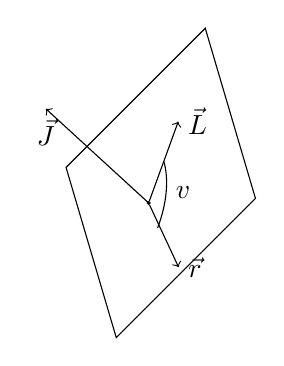
\begin{tikzpicture}[rotate around z=45, rotate around x=-45]
\draw (0,-0.3,0) -- (2.5,-0.3,0) -- (2.5,2.5,0) -- (0,2.5,0) -- cycle;
\draw[->] (1.,1.,0)node[draw,circle,inner sep=0] (o) {} -- (1.5,1.5,2)node[below] {$\vec{J}$};
\draw[->] (o) -- ++(295:0.9cm)node[right] {$\vec{r}$};
\draw[->] (o) -- ++(70:1.1cm)node[right] {$\vec{L}$}node [midway] (aux){};
\draw (aux) arc (0:-50:1) node[midway,right] {$v$};
\end{tikzpicture}

\label{fig:Lenztikz}

\end{figure}

\end{filecontents}%%contain tikz files as filecontents

\addtobeamertemplate{block begin}{\setlength\abovedisplayskip{2pt}\setlength\belowdisplayskip{2pt}\setlength\abovedisplayshortskip{2pt}\setlength\belowdisplayshortskip{2pt}}{}
\addtobeamertemplate{block begin}{\vspace*{-3pt}}{}
\addtobeamertemplate{block end}{}{\vspace*{-3pt}}

\begin{frame}
  \titlepage
\end{frame}

% Section and subsections will appear in the presentation overview
% and table of contents.
%\frame{\tableofcontents[onlyparts]}

\begin{frame}[label={argomenti}]{Fisica stellare: argomenti del corso}
\tableofcontents[onlyparts]
\end{frame}

\begin{wordonframe}{Perch\'e studio queste cose?? Sviluppi; futuro.}

Concretezza, concentrazione, indipendenza

\end{wordonframe}

\part{RegLez}\label{part:intro}
\section{A cosa mi serve?}

\section{RegLez 19}
\begin{frame}[allowframebreaks]{Reg Lez 19}
\begin{itemize}
 \item 18/02/2019 - Introduzione al corso: programma, libri di testo, modalità d'esame, congresso di fotonica. Concetti di base di fisica delle eterostrutture a semiconduttore: tipi di eterostruttura, formalismo della funzione inviluppo, autostati e densità di stati. Pozzi quantici e sottobande; dispersione, elementi di matrice, transizioni interbanda e intersottobanda, regole di selezione.
\item 22/02/2019 - Guadagno in un semiconduttore: elementi di matrice, densità di stati congiunta, condizione di guadagno per i potenziali chimici. Dipendenza da frequenza ed iniezione, effetto della dimensionalità. Dipendenza dalla temperatura e dalla corrente. Meccanismi di iniezione. Resonant tunneling e guadagno in un laser a intersottobanda.
\item 25/02/2019 - Condizione di soglia per cavità Fabry-Perot. Cenni di ottica gaussiana, condizioni di stabilità dei risonatori e diffrazione, casi particolari. Guide d'onda planari: modi TE e TM. Tipi di guide d'onda laser. Fattore di confinamento.
\item 08/03/2019 - Frequenza dei modi laser: gain pulling. Laser multimodo: spectral e spatial hole burning. Laser a semiconduttore: geometrie, materiali, configurazioni. VCSEL e laser in cavità esterna. Laser a quantum wire: tecniche di crescita, proprietà, e prestazioni. Laser a quantum quantum dot: tecniche di crescita, proprietà, e prestazioni. Laser a cascata quantica: guide d'onda, materiali e prestazioni, disegno degli iniettori, laser a singolo modo e stabilizzazione, regioni attive a superreticolo.
\item 11/03/2019 - Laser a cascata quantica: laser multicolori, laser a grandi lunghezze d'onda, guide d'onda a plasmone di superficie, risonatori whispering gallery. Laser THz: regioni attive e guide d'onda, problematiche. Mode-locking: teoria e tecniche (mode-locking passivo, attivo, self-focusing), cenni ai pettini di frequenza.
\item 15/03/2019 - Laser a feedback distribuito: concetto di base, derivazione delle equazioni dei modi accoppiati, condizione di soglia, frequenza dei modi, selettività; caso di coefficiente di accoppiamento reale e immaginario, laser pi-shifted. Laser a emissione verticale: condizione di soglia nei VCSEL, laser DFB del second'ordine.
\item 18/03/2019 - Fotonica terahertz: Auston switches, time-domain spectroscopy, applicazioni di imaging e spettroscopia. Sorgenti THz: photomixers, diodi Gunn e varactors, OPO.
\item 22/03/2019 - Fotonica THz; rivelatori. Modulazione diretta dei laser: oscillazioni di rilassamento e frequenza massima, frequency chirp. Modulatori Stark: principio di funzionamento. Semiconduttori come amplificatori: saturazione, configurazione MOPA.
\item 25/03/2019 - Introduzione alla Fisica dei Materiali 2D; esfoliazione meccanica; ''zoologia'' delle varie famiglie di materiali 2D; eterostrutture di van der Waals; struttura a bande del grafene; elettroni a massa nulla ed equazione di Dirac-Weyl; paradosso di Klein; assorbimento ottico lineare.
\item 28/03/2019 - Trasporto di carica nel grafene; trasporto vicino al punto di Dirac; ''electron-hole puddles'' (EHPs); origine delle EHPs. Teoria dell'assorbimento ottico lineare: assorbimento inter-band universale e assorbimento intra-banda. Teoria di Drude. Bloccaggio di Pauli. Cenni di spettroscopia ARPES. Effetti a molti corpi nello spettro ARPES.
\item 29/03/2019 - Propagazione in un mezzo non lineare: equazioni caratteristiche, problema del phase matching, tecnica del quasi-phase matching. Amplificazione parametrica e oscillatori parametrici: guadagno, condizione di soglia, accordabilità.
\item 01/04/2019 - Modulatori elettro-ottici: cristalli birifrangenti, polarizzazione ordinaria e straordinaria, regime di linearità, limitazioni alla velocità (transit time), modulatori in linea di trasmissione e SAW. Controlo coerente dell'assorbimento: CPA, CPT, sistemi in strong-coupling, sistemi 2D, simmetria PT.
\item 05/04/2019 - Microcavit\'a: Hamiltoniana di Jaynes-Cummings, oscillazioni di Rabi di vuoto e splitting di Rabi di vuoto. Primi esperimenti, polaritoni eccitonici di cavit\'a, polaritoni intersottobanda. Regime di accoppiamento ultraforte. Modulazione del campo di vuoto.
\item 12/04/2019 - Plasmonica nei limiti ritardati e non ritardati: dalle equazioni di Maxwell alla teoria della risposta lineare. Filosofia dei due diversi approcci; cenni della struttura a bande di bilayer graphene e trilayer graphene; bande piatte in twisted bilayer graphene; altri materiali di Dirac: fenomenologia degli isolanti topologici. Aspetti di materials science: da HgTe a WTe2. Dall'effetto Hall quantistico intero ai quantum spin Hall insulators; grafene artificiale; introduzione alla teoria della risposta lineare, suo significato e utilit\'a; esempio di accoppiamento: potenziale scalare e densit\'a elettronica. 
\item 15/04/2019 - Teoria della risposta lineare, derivazione della formula di Kubo; rappresentazione in termini degli autostati esatti; propriet\'a generali delle funzioni di risposta causali; assorbimento.
\end{itemize}
\end{frame}

\part{Stato solido}\label{part:solidstate}
\input{solidstate}

\part{Laser}\label{part:lasers}
\section{Eterostrutture a semi-conduttore}


\part{Optics}\label{part:optics}
\input{optics}

\part{Plasmonics}\label{part:plasmonics}
\input{plasmonics}

\end{document}